\section{The Application}

The application consists of a number of indipendent nodes that comprise a graph. The communication between nodes strongly relies on a publish/subscribe mechanism useful to  exchange data in a distributed system. 

\subsection{Use cases}

\subsubsection{Initialization}
The application is launched by executing the init.launch file. The Roslaunch tool allows to launch multiple ROS nodes as well as set several parameters for the simulation environment. the initialization process brings up the master node, roscore, the coordinator, the semanticMapInterface and Gazebo.\\
\\
Once initialized, the SemanticMapInterface loads from a specified absolute path the Terminology Box and the Assertions Box as Ontology Models.

\begin{lstlisting}[language=Java]
/**
 * Importing Tbox
 */
 tbox = ModelFactory.createOntologyModel( OntModelSpec.OWL_MEM );
 OntDocumentManager dm_tbox = tbox.getDocumentManager();
 dm_tbox.addAltEntry(SOURCE+TBOX_FILE,"file:"+TBOX_FILE);
 tbox.read(SOURCE+TBOX_FILE,"RDF/XML");

/**
 * Importing Abox
 */
 abox = ModelFactory.createOntologyModel( OntModelSpec.OWL_MEM);
 OntDocumentManager dma = abox.getDocumentManager();
 dma.addAltEntry( SOURCE + ABOX_FILE , "file:" + ABOX_FILE);
 abox.read(SOURCE + ABOX_FILE,"RDF/XML");
\end{lstlisting}

The reasoner API supports the notion of specializing a reasoner by binding it to a set of schema or ontology data using the bindSchema call. The specialized reasoner can then be attached to different sets of instance data using bind calls. It is worth noting that in this project the schema (TBox) and instance (ABox) data were saved in two separate files.

\begin{lstlisting}[language=Java]
Reasoner reasoner = ReasonerRegistry.getOWLReasoner();
reasoner = reasoner.bindSchema(tbox);
OntModelSpec ontModelSpec=OntModelSpec.OWL_MEM_MICRO_RULE_INF;
ontModelSpec.setReasoner(reasoner);
InfModel infmodel = ModelFactory.createInfModel(reasoner,abox);
\end{lstlisting}
This is equivalent to an Ontology Model with Reasoner capabilities
specialized on the ABox.
\begin{lstlisting}[language=Java]
infModel = ModelFactory.createOntologyModel( OntModelSpec.OWL_MEM_MICRO_RULE_INF, abox);
\end{lstlisting}

Typically the ontology languages used with the semantic web allow constraints to be expressed, the validation interface is used to detect when such constraints are violated by some data set. The InfModel.validate() interface performs a global check across the schema and instance data looking for inconsistencies. 


\begin{lstlisting}[language=Java]
/** 
 * Consistency Check. Returns true if passed
 */
 private static boolean performConsistencyCheckWith(InfModel inf) {
 boolean res = false; 

 ValidityReport validity = inf.validate();
 if (validity.isValid()) {
	System.out.println(""+ NODE_NAME + "\tConsistency Check:\n Passed\n");
	res = true;
 } else {
	System.out.println(""+ NODE_NAME + "\tConsistency Check:\n Conflicts\n");
	for (Iterator i = validity.getReports(); i.hasNext(); ) {
	    System.out.println(" - " + i.next());
	}
 }
 return res;
}
\end{lstlisting}

When the Coordinator is initialized it sends on a topic called Bridge an init request. The request is captured by the SemanticMapInterface and the $getAllInstances(OntModel)$ method is called. 

\begin{figure}[H]
\centering
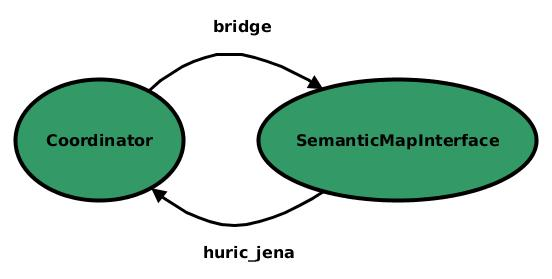
\includegraphics[width=0.8\textwidth]{imgs/topics1.jpg}
\label{fig:actions}
\caption{Data exchange between Coordinator and SemanticMapInterface}
\end{figure}


A collection of instances is retrieved and saved in a HashMap. This method performs the following SPARQL query which returns all Furniture and Drink\footnote{Furniture and Drink are classes defined in the Terminology Box} entities. 

\begin{lstlisting}[language=Java]
String queryString = "PREFIX rdf: <http://www.w3.org/1999/02/22-rdf-syntax-ns#>" +
				"prefix rdfs: <"+RDFS.getURI()+">\n" +
	    		"PREFIX xsd: <http://www.w3.org/2001/XMLSchema#> " +
	    		"PREFIX hasPosition: <" + NS + POSITION +"> " +
	    		"PREFIX hasRef: <" + NS + PREF_REF +"> " +
				"prefix semantic_mapping_domain_model: <" + DOMAIN_MODEL_NS + "#> \n"+
				"prefix semantic_mapping_1: <" + SEMANTIC_MAP_NS + "#> \n"+
	    		
	    		"PREFIX coordx: <" + NS + COORD_X +"> " +
	    		"PREFIX coordy: <" + NS + COORD_Y +"> " +
	    		"PREFIX coordz: <" + NS + COORD_Z +"> " +
	    		"PREFIX prefRef: <" + NS + LEXICAL +"> " +
	    		
	    		
	    		"SELECT DISTINCT ?uri ?class ?x ?y ?z ?lex "+
	    		"WHERE {" + 
	    			"{"+
		    		"?uri a ?class ." + 
		    		"?class rdfs:subClassOf semantic_mapping_domain_model:Furniture ."+
		    		"?uri hasPosition: ?pos ." + 
		    		"?uri hasRef: ?ref ." + 
		    		"?ref prefRef: ?lex ." + 
		    		"?pos coordx: ?x . " + 
		    		"?pos coordy: ?y . " + 
		    		"?pos coordz: ?z " +  "} UNION {"+
		    		"?uri a ?class ." + 
		    		"?class rdfs:subClassOf semantic_mapping_domain_model:Drink ." +
		    		"?uri hasPosition: ?pos ." + 
		    		"?uri hasRef: ?ref ." + 
		    		"?ref prefRef: ?lex ." + 
		    		"?pos coordx: ?x . " + 
		    		"?pos coordy: ?y . " + 
		    		"?pos coordz: ?z " +  "}"+
"}" ;
\end{lstlisting}
The resulting information are embedded in a message and sent on a topic called \textit{Huric\_jena}. The Coordinator Node receives and parses the message. 

The communication between Gazebo and the Coordinator uses services which are defined as pair of messages: one for the request and one for the reply. A providing ROS node offers a service under a string name, and a client calls the service by sending the request message and awaiting the reply.

Once the reponse from the SemanticMapInterface has been received, the Coordinator calls a special service that allows to create and render 3D models dynamically in the simulation environment of Gazebo.


\begin{figure}[H]
\centering
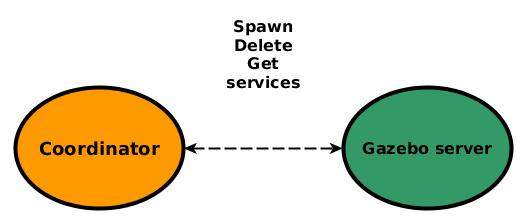
\includegraphics[width=0.5\textwidth]{imgs/gazebocoord.jpg}
\label{fig:actions}
\caption{Data exchange between the Coordinator and Gazebo}
\end{figure}



\subsubsection{Insertion of entities}
\label{subsec: insertion}
Considering a real world scenario in which a perception node recognizes an object from a stream of a point cloud data, instances of a given class should be dynamically inserted in the Assertion Box by publishing a predefined command on a topic.\\
One node can create an instance by specifying its super class, its spacial positions and preferred lexical reference. Another faster way include the possibility to add a Chair in fixed position. These insertion methods are issued by the ExternInterface node, captured by the Coordinator and forwarded to the SemanticMapInterface.


\begin{figure}[H]
\centering
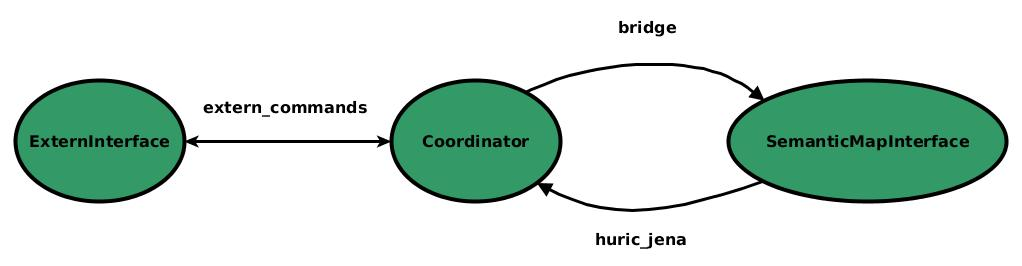
\includegraphics[width=0.8\textwidth]{imgs/topics2.jpg}
\label{fig:actions}
\caption{Data exchange between ExternInterface, Coordinator and SemanticMapInterface}
\end{figure}


The Java Node provides two methods to insert an instance of given type into the ontology model loaded in memory:
\begin{itemize}
\item Triple manipulation based
\item SPARQL based
\end{itemize}
Jena Ontology API provides a full set of methods to manipulate statements. The handleAddEntityRequest(ontModel,ontClass, uri, pose,lexicalReference) method is given below:

\begin{lstlisting}[language=Java]
/**
 * Handles AddEntityRequests from orchestrator using Jena API
 *	Creates a new instance, adds properties to it and perform consistency check
 * If test is passed, leaves the newly created instance, otherwise deletes it
 */
	private static boolean handleAddEntityRequest(OntModel abox, OntClass ontClass, String uriInstance, String posX,
			String posY, String posZ, String lexicalReference){
		boolean res = false;

	    OntClass prefrefClass = abox.getOntClass(NS+PREF_REF_CLASS);
	    OntClass coordinatesClass = abox.getOntClass(NS+COORDINATES_CLASS);

		String uriBase = "http://www.semanticweb.org/ontologies/2016/1/semantic_mapping_1#";
		// Create instance
	    //OntClass class1 = abox.getOntClass(NS+ontClass);
		
		if (ontClass == null)
			return false;
		else {
			// Create Individuals
			Individual i1 = abox.createIndividual(uriInstance,ontClass);
		    Individual prefRefInd = abox.createIndividual(uriBase+lexicalReference
		    +"_pref_ref",prefrefClass);
		    Individual coordinatesInd = abox.createIndividual(uriBase+lexicalReference
		    +"_pref_ref",coordinatesClass);
			
			
		    // Create Datatype Property
		    DatatypeProperty lexicalRef = abox.getDatatypeProperty(NS + LEXICAL);
			Literal ref = abox.createTypedLiteral(lexicalReference);
			Statement refStatement = abox.createStatement(prefRefInd, lexicalRef, ref);
			abox.add(refStatement);
			
			//  Bind pref reference individual to object individual
			ObjectProperty hasPrefRef = abox.getObjectProperty(NS+PREF_REF);
			Statement bindPrefRef = abox.createStatement(i1, hasPrefRef, prefRefInd);
			abox.add(bindPrefRef);
			

		    // Create Datatype Property for coordinate X
		    DatatypeProperty posx = abox.getDatatypeProperty(NS + COORD_X);
			Literal posXFloat = abox.createTypedLiteral(posX);
			Statement posXStatement = abox.createStatement(coordinatesInd, posx, posXFloat);
			abox.add(posXStatement);
		    // Create Datatype Property for coordinate X
		    DatatypeProperty posy = abox.getDatatypeProperty(NS + COORD_Y);
			Literal posYFloat = abox.createTypedLiteral(posY);
			Statement posYStatement = abox.createStatement(coordinatesInd, posy, posYFloat);
			abox.add(posYStatement);
		    // Create Datatype Property for coordinate X
		    DatatypeProperty posz = abox.getDatatypeProperty(NS + COORD_Z);
			Literal posZFloat = abox.createTypedLiteral(posZ);
			Statement posZStatement = abox.createStatement(coordinatesInd, posz, posZFloat);
			abox.add(posZStatement);
			

			//  Bind position individual to object individual
			ObjectProperty hasPosition = abox.getObjectProperty(NS+POSITION);
			Statement bindPose = abox.createStatement(i1, hasPosition, coordinatesInd);
			abox.add(bindPose);
			
			// Now perform consistency check

		    InfModel infModel = ModelFactory.createOntologyModel( OntModelSpec.OWL_MEM_MICRO_RULE_INF, abox);
			res = performConsistencyCheckWith(infModel);
		}
		
		return res;
}
\end{lstlisting}

The second method is called AddEntityRequest(abox,ontclass,uri,pose,lexicalReference) and it is based on a SPARQL query:

\begin{lstlisting}[language=Java]
/**
 * Handles AddEntityRequests using SPARQL
 *	Creates a new instance, adds properties to it and perform consistency check
 * If test is passed, leaves the newly created instance, otherwise deletes it
 */
 private static boolean AddEntityRequest(OntModel abox, OntClass ontClass, String uriInstance, String posX,
			String posY, String posZ, String lexicalReference){
 boolean res = true;
		
 String uri_Instance[] = uriInstance.split("#");
		
 if (ontClass == null) {
    res = false;
	System.out.print("\n"+ NODE_NAME + "\t[ Add Entity ] Class problem\n");
 } else {
			String queryString = "" + 
			"prefix rdfs: <"+ RDFS.getURI() +">\n" +
			"prefix rdf: <http://www.w3.org/1999/02/22-rdf-syntax-ns#> \n"+
			"PREFIX xsd: <http://www.w3.org/2001/XMLSchema#> "
			
			+ "prefix semantic_mapping_domain_model: <" + DOMAIN_MODEL_NS + "#> \n"
			+ "prefix semantic_mapping: <" + SEMANTIC_MAP_NS + "#> \n"
			+ "PREFIX class: <"+ ontClass.getURI() +">\n"
			
			
			+ "insert data { semantic_mapping:"+uri_Instance[1] +" rdf:type class: . "
			
			
			// Add hasPosition Irreflexive ObjectProperty 
			+ "semantic_mapping:" + uri_Instance[1] + " semantic_mapping_domain_model:hasPosition semantic_mapping:" + uri_Instance[1]
			+ "_coordinates . " 
			
			// Add Instance Coordinates 
			+ "semantic_mapping:" + uri_Instance[1]+ "_coordinates rdf:type semantic_mapping_domain_model:Coordinates . " 

			// Add datatype Property
			+ "semantic_mapping:" + uri_Instance[1] + "_coordinates semantic_mapping_domain_model:float_coordinates_x \""
			+ posX + "\"^^xsd:float . "
			+ "semantic_mapping:" + uri_Instance[1] + "_coordinates semantic_mapping_domain_model:float_coordinates_y \"" + posY
			+ "\"^^xsd:float . "
			+ "semantic_mapping:" + uri_Instance[1] + "_coordinates semantic_mapping_domain_model:float_coordinates_z \"" + posZ
			+ "\"^^xsd:float . "

			// Add hasPreferredReference ObjectProperty
			+ "semantic_mapping:" + uri_Instance[1] + " semantic_mapping_domain_model:hasPreferredReference semantic_mapping:" + uri_Instance[1]
			+ "_preferredReference . " 

			// Create Instance Lexical Reference
			+ "semantic_mapping:" + uri_Instance[1] + "_preferredReference rdf:type semantic_mapping_domain_model:PreferredReference . "

			+ "semantic_mapping:" + uri_Instance[1] + "_preferredReference semantic_mapping_domain_model:lexicalReference \"" + lexicalReference
			+ "\"^^xsd:string . " + "} \n ";
			
			UpdateAction.parseExecute(queryString, abox);
			
			// Check inconsistencies
		    InfModel infModel = ModelFactory.createOntologyModel( OntModelSpec.OWL_MEM_MICRO_RULE_INF, abox);
			res = performConsistencyCheckWith(infModel);
		}
	
		return res;
}
\end{lstlisting}

Once the instance has been inserted into the ontology model, the collection of new entities is once again sent on the \textit{huric\_jena} topic and captured by the coordinator which invokes the Gazebo service to render the 3D model of the newly created instances at the provided position in space.


\subsubsection{Deletion of an entity}
\label{subsubsec:delete}
In a real world scenario, objects can move or be manipulated by humans. A delete function is needed in order to handle cases in which the object moves out of the field of perception of the robot. To delete a model a special routine is invoked.\\
The request is published on the external\_commands topic and captured by the Coordinator. This node forwards the request to SemanticMapInterface node and waits for the response. If the abox has been correctly updated, it invokes the delete\_model service exposed by the Gazebo node. The resulting 3D environment is consistent with the instance data loaded in memory.

The SemanticMapInterface provides a method the handle this request. In Section \ref{subsec:abox} we have seen that for each furniture object there is an linear position and lexical reference instance associated with it. In order to completely delete a furniture object, these instances have to be canceled as well. The query that handles this operation is in the Listing below.
\begin{lstlisting}[language=Java]
/**
  * Handles removeEntityRequests from orchestrator:
  *	Looks for an instance with uri 'uriInstance', if the instance does not exist returns false.
  * If there is match, it deletes it and returns true. 
  * 
  * Attention : What happens if an instance of a master concept relating two entities is deleted?
  * 			No one should be able to alter its knowledge directly.
  *	
  * 			Maybe, add a negative weight to the instance or a tag
  */
private static boolean handleRemoveEntityRelatedRequest(OntModel abox, String uriInstance) {
	boolean res = false;

	String uri_Instance[] = uriInstance.split("#");
	//  Removing IS A statement
	String queryStringDelete = "" + 
			"prefix rdfs: <"+RDFS.getURI()+">\n" +
			"prefix rdf: <http://www.w3.org/1999/02/22-rdf-syntax-ns#> \n"+
			"PREFIX xsd: <http://www.w3.org/2001/XMLSchema#> "				
			+ "prefix semantic_mapping_domain_model: <" + DOMAIN_MODEL_NS + "#> \n"
			+ "prefix semantic_mapping: <" + SEMANTIC_MAP_NS + "#> \n"
			+ "delete { semantic_mapping:"+uri_Instance[1] +" ?pred ?obj }  "
        + "where { semantic_mapping:"+uri_Instance[1] + " ?pred ?obj }";
			
			UpdateAction.parseExecute(queryStringDelete, abox);
	

	//  Removing coordinates statement
	String queryStringPosDelete = "" + 
			"prefix rdfs: <"+RDFS.getURI()+">\n" +
			"prefix rdf: <http://www.w3.org/1999/02/22-rdf-syntax-ns#> \n"+
			"PREFIX xsd: <http://www.w3.org/2001/XMLSchema#> "				
			+ "prefix semantic_mapping_domain_model: <" + DOMAIN_MODEL_NS + "#> \n"
			+ "prefix semantic_mapping: <" + SEMANTIC_MAP_NS + "#> \n"
			+ "delete { semantic_mapping:"+uri_Instance[1] + "_coordinates ?pred ?obj }  "
        + "where { semantic_mapping:"+uri_Instance[1] + "_coordinates ?pred ?obj }";
			
			UpdateAction.parseExecute(queryStringPosDelete, abox);
	
	String queryStringRefDelete = "" + 
			"prefix rdfs: <"+RDFS.getURI()+">\n" +
			"prefix rdf: <http://www.w3.org/1999/02/22-rdf-syntax-ns#> \n"+
			"PREFIX xsd: <http://www.w3.org/2001/XMLSchema#> "				
			+ "prefix semantic_mapping_domain_model: <" + DOMAIN_MODEL_NS + "#> \n"
			+ "prefix semantic_mapping: <" + SEMANTIC_MAP_NS + "#> \n"
			+ "delete { semantic_mapping:"+uri_Instance[1] + "_preferred_reference ?pred ?obj }  "
        + "where { semantic_mapping:"+uri_Instance[1] + "_preferred_reference ?pred ?obj }";
			
			UpdateAction.parseExecute(queryStringRefDelete, abox);
			
	return res;
}
\end{lstlisting}
\label{lst:delete}

\subsubsection{Update entity's properties}
The system provides an update function to modify properties of an existing entity in the ABox. By publishing a formatted command on the extern\_commands topic, the Coordinator node forwards the request to the SemanticMapInterface. The method responsible for the update is called handleUpdateEntityRequest(abox,ontClass, uriInstance, posX, posY, posZ,  lexicalReference).

\begin{lstlisting}[language=Java]
/**
  * Handles updateEntityRequests using SPARQL
  *	Looks for an instance with uri 'uriInstance', if the instance does not exist returns flase.
  * If there is match, it looks for the properties Pose and LexicalReference and updates it. 
  * A consistency if invoked. If the test is passed, true is returned. Otherwise False.
  */
private static boolean handleUpdateEntityRequest(OntModel abox,OntClass ontClass,
 String uriInstance, String posX,
		 String posY, String posZ, String lexicalReference) {
	boolean res = false;

	System.out.println(""+ NODE_NAME + "\tDeleting Instance " + uriInstance);
	handleRemoveEntityRelatedRequest(abox,uriInstance);

	System.out.print("\n"+ NODE_NAME + "\tNow inserting: "+ posX + ", " + posY + " , " + posZ);
	if (AddEntityRequest(abox,ontClass,uriInstance,posX,posY,
	posZ,lexicalReference)) {
	System.out.println("\n"+ NODE_NAME + "\tInstance inserted successfully");
	res = true;
   	} else {
    		System.out.print(""+ NODE_NAME + "\tError could not insert instance consistency problem");
    	}
	
	return res;
}
\end{lstlisting}

The update routine starts by looking for an instance with the provided uri. If the there is no match, false is returned. Then it deletes the instance itself and its related properties with the method presented in Section \ref{subsubsec:delete}. Finally the new instance is added by invoking the method discussed in Section \ref{subsec: insertion} and a consistency check is invoked. 

It is also possible to update an instance by dragging it in the 3D environment of Gazebo. The coordinator node keeps track of the position of all instances and compare them with the corresponding coordinate properties in the Assertion Box. As soon as the position of an instance is modified and a predefined threshold is crossed, an update routine is triggered and the ABox is updated. Collisions have not been taken into account.

\subsection{Exporting Ontology}
Human machine interfaces require a context-aware interaction. In this process, since both parts make references to real world objects, an ontological model of the environment and a description of the involved entities may help in improving the accuracy of the interpretation of an user utterance.\\
The first step towards this direction is to provide an export feature that allows the robotic platform to be aware of the surrounding environment and nearby objects.\\
\\

\begin{lstlisting}[language=Java]
/** 
  * Exports Ontology if consistency check passed
  */
private static boolean exportTo(InfModel inf, OntModel abox, String absolutePath, String fileName){
	boolean res = false;
	if (performConsistencyCheckWith(inf)) {
		exportOntologyOnt(abox,absolutePath,fileName);
		res = true;
	}
	else {
		res = false;
	}
	return res;
}

/** 
  * Exports Ontology to a file with provided name and path.
  */
private static boolean exportOntologyOnt(OntModel inf, String absoluteFileName, String fileName){
	boolean res = false;
    FileWriter out = null;

    	try{
    		out = new FileWriter(absoluteFileName+fileName);
    		inf.write(out,"RDF/XML-ABBREV");
    		res = true;
	    	System.out.println(""+ NODE_NAME + "\tConsistency check passed. Writing to file:\t"+fileName);
    	}
    	catch (IOException a){
    		System.out.println(""+ NODE_NAME + "\tExport Problem");
            a.printStackTrace();
    	}
    	finally{
    		if (out!=null){
    			try {out.close();} catch(IOException ex) {}
    		}
    	}

    	return res;
}
\end{lstlisting}

The SemanticMapInterface export the ontology to OWL file in the file system and sends the list of entities to the Coordinator Node.

\subsubsection*{Listing Entities}
\label{subsubsec:list}
In order to retrieve the list of entities perceived by the robot, another feature has been taken into account. This action involves the Coordinator, the SemanticMapHandler and the ExternInterface nodes. The Coordinator prepares the response in two formats, a json encoded list of entities and corresponding properties

\begin{lstlisting}[language=Java]
{
   "http://www.semanticweb.org/ontologies/2016/1/semantic_mapping_1#table1":{
      "type_full":"http://www.semanticweb.org/ontologies/2016/1/
      semantic_mapping_domain_model#Table",
      "coordinates":"2.0,2.0,0.0",
      "preferredLexicalReference":"table",
      "atom":"table1",
      "coordinate":{
         "y":"2.0",
         "x":"2.0",
         "z":"0.0"
      },
      "type":"Table"
   },{
   ...
   },
   "http://www.semanticweb.org/ontologies/2016/1/semantic_mapping_1#beer_can_1":{
      "type_full":"http://www.semanticweb.org/ontologies/2016/1
      /semantic_mapping_domain_model#Beer",
      "coordinates":"1.8,2.2,1.0",
      "preferredLexicalReference":"Beer",
      "atom":"beer_can_1",
      "coordinate":{
         "y":"2.2",
         "x":"1.8",
         "z":"1.0"
      },
      "type":"Beer"
   }
}
\end{lstlisting}


and human readable output for debug purposes.  




\subsection{Future works}

The application supports a limited number of entity types. Each instance has to be associated with its corresponding 3D model and inertia matrix. In this project four types of objects are supported: tables, chairs, beer and coke cans.

From a robotic perspective, the applications of this ROS package are related to Human Centered Robotics.

\subsubsection*{LU4R - Adaptive spoken Language Understanding For Robots}
The adaptive spoken Language Understanding chain For Robots tool is the result of the collaboration between the SAG group at Tor Vergata University of Rome and the Laboratory of Cognitive Cooperating Robots (Lab.Ro.Co.Co.) at Sapienza, University of Rome. LU4R\footnote{For further information visit the official web page at http://sag.art.uniroma2.it/lu4r.html} receives as input one or more transcriptions of a spoken command and produces an interpretation that is consistent with a linguistically-justified semantic representation, coherent with the perceived environment. LU4R is based on a spoken language understanding (SLU) process that integrates perceptual and linguistic information in order to produce command interpretations that coherently express constraints about the world and the hosting robotic platform.\\
\\
It is a ROS compatible Java application in which the client runs on the robotic platform and the server on a remote machine.\\
Actions expressed in user utterances can be modeled as semantic frames, sentences expressing commands are automatically analyzed by the chain by applying data driven methods trained over the Human Robot Interaction Corpus (HuRIC)\cite{bib3}.
\\
In its default mode of operation, the chain requires a list of sentences paired with their transcription confidence score and the ranking position among the hypotheses list. In order to enable the environment based interpretation process, additional information are required. The json described in Section \ref{subsubsec:list} can be forwarded to the LU4R node.
%In order to react to a user command a number of implicit assumptions should be made. 

%The correct interpretation of the spoken sentences depends on the physical, cognitive and linguistic aspects triggered by the operational environment.

%``take the book on the table ''

%First, at least two entities, a book and a table, must exist in the environment and the speaker must be aware
%of such entities. Accordingly, the robot must have access to
%an inner representation of the objects, e.g. an explicit map of
%the environment.
%The perception of the environment that explicitly affects linguistic reasoning.
%In the ontology based approach, OWL is used to model a Reference Ontology, while RDFS  is used  to  model schemas  to  be mapped. 